\section{Concluding remarks}\label{sec:remarks}

\subsection{How far can the method go?}\label{sec:limits}

A relaxation can never prove a bound below $\muR$. Romik's shape turns monotonically through every orientation between $0\dg$ and $90\dg$ in both turns, so for all finite $A,B\subset[0\dg,90\dg]$ it lies in an intersection of the kind used in \cref{def:G}, by \cref{lem:frame}, and \cref{lem:relax} gives $G(A;B)\ge\muR$.

For the relaxation of \cref{thm:computation}, the hallway positions taken by Romik's motions at the orientations $\alpha_1$ and $\alpha_2$ give a connected intersection of area $1.7229\ldots$ (\cref{fig:relax}(a)). A local search over the eight parameters, in floating-point arithmetic, found the larger configuration of \cref{fig:relax}(b). Rounded to four decimals, its parameters are $\bu_{\alpha_1}=\bv_{\alpha_1}=(0.1260,\,0.4425)$ and $\bu_{\alpha_2}=\bv_{\alpha_2}=(0.1322,\,0.5397)$. For these values the intersection in \eqref{eq:G} is connected and has area $29{,}092{,}957{,}301/16{,}800{,}000{,}000=1.73172\ldots$, as we checked in exact rational arithmetic with the routines of the Python checker. Hence $1.7317<G(\{\alpha_1,\alpha_2\};\{\alpha_1,\alpha_2\})\le\Tmain$, and the bound of \cref{thm:computation} cannot be pushed below $1.7317$.

\begin{figure}[h]
\centering
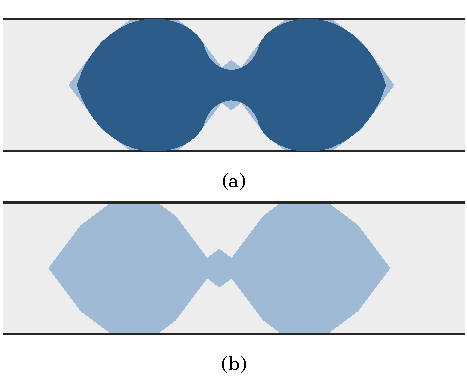
\includegraphics[width=0.66\textwidth]{figures/fig_relax.pdf}
\caption{The relaxation of \cref{thm:computation}. (a) Romik's shape $\Sigma$ (dark) inside the intersection of $H$ with the four hallways at the positions taken by Romik's motions at the orientations $\alpha_1$ and $\alpha_2$ (light); the intersection has area $1.7229\ldots$. (b) The configuration found by local search; the intersection has area $1.7317\ldots$. In both cases the intersection is connected.}
\label{fig:relax}
\end{figure}


\needspace{5\baselineskip}
The size of the certificate grows quickly as the threshold decreases (\cref{tab:growth}). No certificate exists for $T$ below the value of the relaxation, so one expects the number of nodes to grow without bound as $T$ decreases towards that value, or towards a somewhat larger one if the estimates on boxes are too weak.

\begin{table}[ht]
\centering
\caption{Size of the certificate for $G(\{\alpha_1,\alpha_2\};\{\alpha_1,\alpha_2\})\le T$ found by the search, for several thresholds $T$.}
\label{tab:growth}
\begin{tabular}{@{}lrrrrr@{}}
\toprule
$T$ & $1.85$ & $1.80$ & $1.78$ & $1.77$ & $1.765$ \\
\midrule
Nodes (millions) & $5.1$ & $41.2$ & $171.1$ & $475.2$ & $872.3$ \\
\bottomrule
\end{tabular}
\end{table}

Other choices of two angles on each side, including unequal sets $A\neq B$, gave local-search values between $1.732$ and $1.769$, no smaller than for $\{\alpha_1,\alpha_2\}$. Adding angles cannot increase the value of the relaxation, since $G(A';B')\le G(A;B)$ whenever $A\subset A'$ and $B\subset B'$, but it makes the search more expensive. With three angles on each side, for example $\{\alpha_1,\arcsin(119/169),\alpha_2\}$, local search finds configurations of area about $1.7217$, but at the threshold $1.85$ the search needed about six times as many nodes as with two angles.

Kallus and Romik proved that suitable maxima of their relaxations converge to the moving sofa constant as the angles become dense \cite[Theorem~5]{kallusromik2018}; the relaxations used there also constrain the final orientation of the sofa, by a set that contains all rotations of $V$ in a given range of angles. We have not proved the analogous statement for $G(A;B)$ and $\muA$. Even if it holds, our experiments suggest that two angles on each side will not give a bound much below $1.73$, and that more angles will be practical only with better estimates on each box or a reduction of the parameter space by symmetry.

\needspace{5\baselineskip}
\subsection{Open questions}

\begin{enumerate}[label=(\arabic*),leftmargin=*]
\item Is Romik's shape optimal? Is it at least locally optimal among nearby ambidextrous sofas? Romik lists local optimality as an open problem \cite{romik2018}. For numerical evidence and partial results see \cite{mohammed2026,bonfioli2026}.

\item Is $\muZ(D)$ equal to $\muA$ for all sufficiently large $D$?

\item Is $G(\{a\};\{a\})=\sec a+\csc a-\csc2a$ for all $a\in(0\dg,90\dg)$? At $a=45\dg$ this is \cref{prop:onehalf}. For $a=30\dg,35\dg,\dots,60\dg$, numerical local search from many random starting points reached this value to ten digits and never exceeded it. It would be the ambidextrous counterpart of the value $G_{(a)}=\sec a+\csc a$ for the ordinary problem \cite[Section~2]{kallusromik2018}.

\item Kallus and Romik showed that a moving sofa of maximal area must rotate by at least $81.2\dg$ \cite[Theorem~2]{kallusromik2018}. \Cref{prop:natural} shows that an ambidextrous sofa of area greater than $T$ rotates by at least $\gamma_T$ in each turn. Can the method of \cref{sec:method} show that ambidextrous sofas of area close to $\muA$ rotate substantially further?
\end{enumerate}
